\documentclass[a4paper, 12pt, margins=3cm]{homework}
\usepackage{tikz}

\usepackage{graphicx}
\usepackage{dsfont}
\usepackage{microtype}
\usepackage{mathrsfs}
\usepackage[ngerman]{babel}
\usepackage{csquotes}
\usepackage[T1]{fontenc}
\usepackage{lmodern}
\usepackage{wasysym}

\setlength{\parindent}{0pt}

\newcommand{\R}{\mathbb{R}}
\newcommand{\N}{\mathbb{N}}
\newcommand{\Z}{\mathbb{Z}}
\newcommand{\Q}{\mathbb{Q}}
\newcommand{\C}{\mathbb{C}}

\name{Tobias Eidelpes}
\course{Algebra und Diskrete Mathematik}
\term{2015WS}
\hwnum{7}
\hwtype{Übungsblatt}
\problemtitle{Aufgabe}
\solutiontitle{Lösung}

\begin{document}
  \begin{center}
    \textsc{Beispiele 212, 220, 228, 235, 254, 315, 320}
  \end{center}


% AUSSTÄNDIG 212
  \problemnumber{212}
  \begin{problem}
    Gesucht ist die allgmeine Lösung der linearen Differenzengleichung
    \[ x_{n+1} = 3^{2n}x_n+3^{n^2}, \quad n = 0,1,2... \]
  \end{problem}
  \begin{solution}
    Diese Art der Differenzengleichung bezeichnet man als \emph{allgemeine 
    lineare Differenzengleichung erster Ordnung} der Form $x_{n+1} = a_n x_n + b_n$
    Daraus folgt folgendes Kochrezept:
    \begin{enumerate}\itemsep0pt
      \item Suche Lösung der homogenen Gleichung $x_{n+1} = a_nx_n$, die homogene
      Lösung $x_n^{(h)}$.
      \item Suche eine Lösung der inhomogenen Gleichung $x_{n+1} = a_nx_n+b_n$,
      die sogenannte partikuläre Lösung $x_n^{(p)}$, z.B. mittels Variation der
      Konstanten.
      \item Bilde die Lösungsgesamtheit durch $x_n = x_n^{(h)} + x_n^{(p)}$.
    \end{enumerate}
    \subsection*{Homogene Lösung}
  \end{solution}


% ERLEDIGT 220
  \problemnumber{220}
  \begin{problem}
    Gesucht sind die allgemeinen Lösungen der linearen homogenen Differenzengleichungen
    \begin{parts}
      \part \label{220.a}
      $x_{n+2} + 12x_{n+1} + 36x_n = 0$
      \part \label{220.b}
      $x_{n+2} - 2x_{n+1} + 5x_n = 0$
      \part \label{220.c}
      $x_{n+2} + 11x_{n+1} + 28x_n = 0$
    \end{parts}
  \end{problem}
  \begin{solution} \hfill

    \ref{220.a}
      Charakteristische Gleichung: 
      \[ \lambda^2 + 12\lambda + 36 = 0 \]
      Die Nullstellen dieser Funktion sind:
      \[ -\frac{p}{2} \pm \sqrt{\frac{p^2}{4} - q} = -6 \pm \sqrt{36-36} = \lambda_1 = \lambda_2 = -6 \]
      Allgemeine Lösung:
      \[ x_n = \lambda_1 \cdot (-6)^n + \lambda_2 \cdot n \cdot (-6)^n = (-6)^n \cdot (C_1 + C_2 \cdot n) \]

  \newpage
    
    \ref{220.b}
      Charakteristische Gleichung:
      \[ \lambda^2 - 2\lambda + 5 = 0 \]
      Die Nullstellen dieser Funktion sind:
      \[ +1 \pm \sqrt{-4} = 1 \pm 2i \]
      \[ \lambda_1 = 1 + 2i \qquad \lambda_2 = 1 - 2i\]
      Umwandlung in Polarkoordinaten:
      \[ r = \sqrt{1+2^2} = \sqrt{5}, \quad \varphi = atan(\frac{2}{1}) \approx 1.11 \]
      Daraus die allgemeine Lösung:
      \[ x_n = (\sqrt{5})^n \cdot (D_1 \cdot cos(1.11n) + D_2 \cdot sin(1.11n)) \]
    \ref{220.c}
      Charakteristische Gleichung:
      \[ \lambda^2 + 11\lambda + 28 = 0 \]
      Die Nullstellen dieser Funktion sind:
      \[ \lambda_1 = -7 \qquad \lambda_2 = -4 \]
      Allgemeine Lösung: 
      \[ x_n = C_1 \cdot (-7)^n + C_2 \cdot (-4)^n \]
  \end{solution}


% AUSSTÄNDIG 228
  \problemnumber{228}
  \begin{problem}
    Berechnen Sie die folgende Summe durch Aufstellen und Lösen einer Rekursion
    mittels Ansatzmethode.
    \[ \sum_{i=1}^n{i(i-1)} \]
  \end{problem}
  \begin{solution}
    
  \end{solution}


% AUSSTÄNDIG 235
  \problemnumber{235}
  \begin{problem}
    Lösen Sie die Rekursion mit der Ansatzmethode:
    \[ a_n + a_{n-1} + a_{n-2} = 1 + sin(n\frac{\pi}{3}) \; (n \geq 2), a_0 = 3, a_1 = -1 \]
  \end{problem}
  \begin{solution}
    
  \end{solution}


% ERLEDIGT 254
  \problemnumber{254}
  \begin{problem}
    Stellen Sie eine Rekursion für die gesuchten Zahlen $a_n$ auf und lösen Sie diese: \\

    $a_n$ sei die Anzahl aller 0-1-Folgen der Länge $n$, in denen es keine benachbarten
    Nullen gibt.
  \end{problem}
  \begin{solution}
    $a_1 = 2$, weil es zwei Möglichkeiten an Bitfolgen der Länge 1 gibt (0 und 1).
    $a_2 = 3$, weil es drei Möglichkeiten an Bitfolgen der Länge 2 gibt (01, 10, 11).
    Für $n \geq 3$ endet so eine Bitfolge entweder mit einer 1 oder mit einer 0.
    Das heißt, wenn das $n$-te Bit 1 ist, liefern die vorangehenden $n-1$ Bits
    bereits durch $a_{n-1}$ erfasste Folgen; falls das $n$-te Bit 0 ist, müssen
    die letzten beiden Bits 10 sein und die vorangehenden $n-2$ Bits bilden eine
    Folge, die durch $a_{n-2}$ mitgezählt wird. Daraus folgt:
    \[ a_n = a_{n-1} + a_{n-2} \qquad n\geq 3 \text{ mit } a_1 = 2 \text{ und } a_2 = 3 \]
  \end{solution}


% ERLEDIGT 315
  \problemnumber{315}
  \begin{problem}
    Man bestimme im folgenden Graphen $H$ für den angegebenen Wert von $x$ mit
    Hilfe des Kruskalalgorithmus einen minimalen und einen maximalen spannenden
    Baum.\\

    \centering 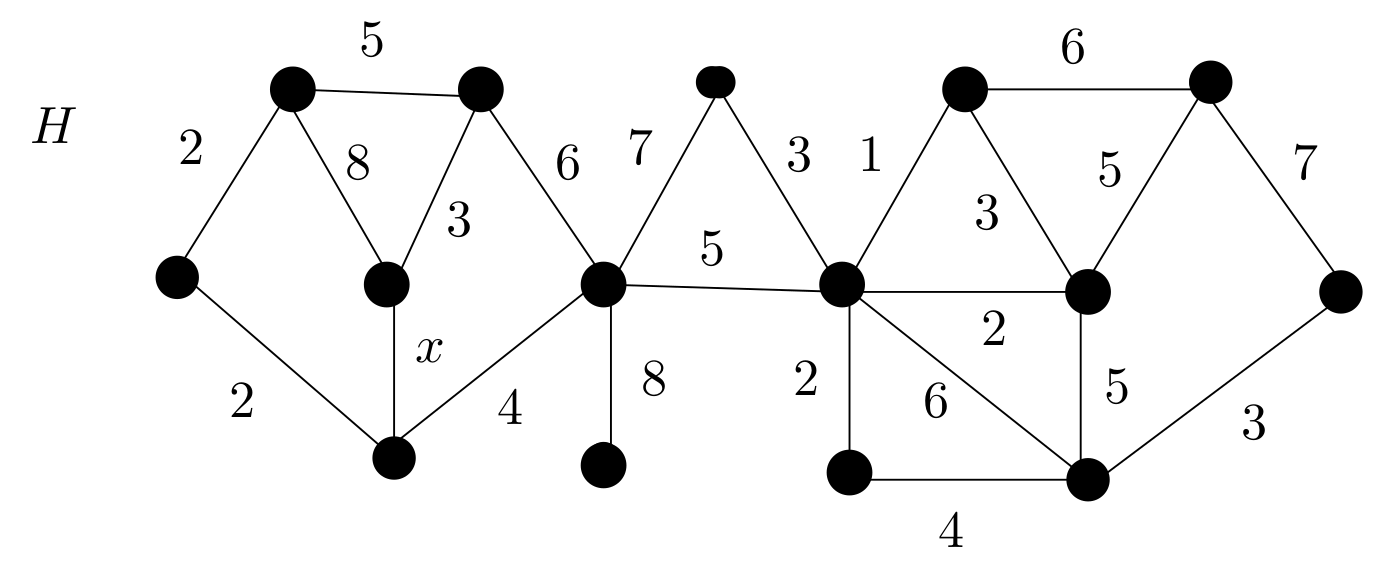
\includegraphics[scale=0.2]{315.png}
    \[ x = 2 \]
  \end{problem}
  \begin{solution}
    Minimaler Spannbaum: \\

    \begin{center}
      \def\svgwidth{300pt} \input{315minimal.pdf_tex}
    \end{center}

    Maximaler Spannbaum: \\

    \begin{center}
      \def\svgwidth{300pt} \input{315maximal.pdf_tex}
    \end{center}
  \end{solution}


% ERLEDIGT 320
  \problemnumber{320}
  \begin{problem}
    Im nachstehenden bewerteten Graphen bestimme man mit Hilfe des Dijkstra-Algorithmus
    einen Entfernungsbaum bezüglich des Knoten $v_0$. \\

    \centering 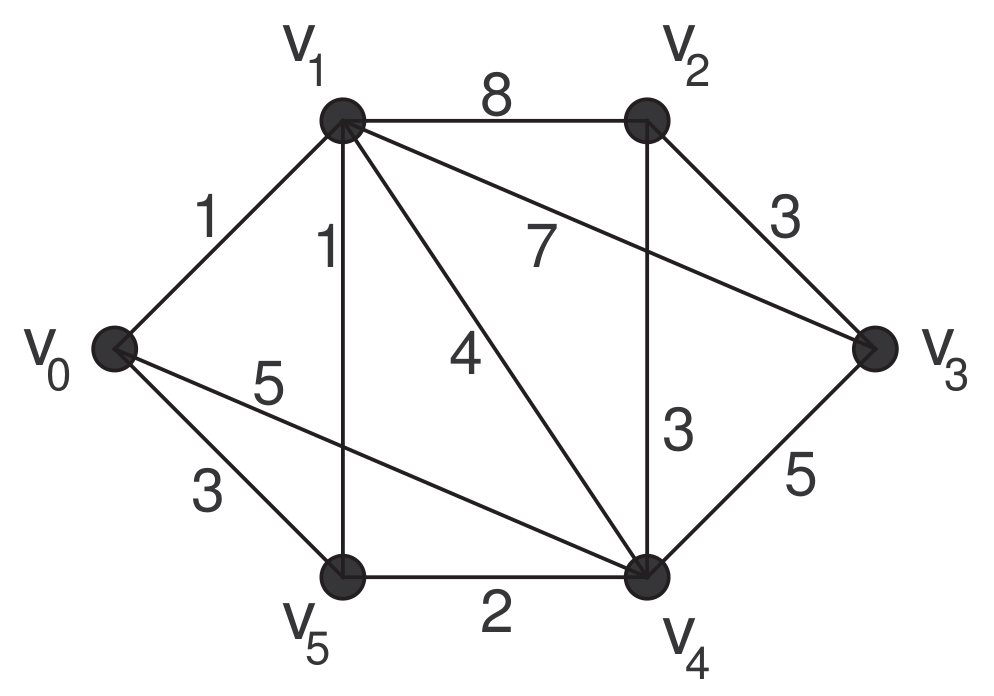
\includegraphics[scale=0.2]{320.png}
  \end{problem}
  \begin{solution} \hfill 
    \begin{center}
      \def\svgwidth{300pt} \input{320.pdf_tex}
    \end{center}
  \end{solution}
\end{document}